\documentclass{article}
\usepackage{amsmath}
\usepackage{amssymb}
\usepackage{geometry}
\geometry{a4paper, margin=1in}
\usepackage{graphicx}
\usepackage{float}

\title{Esercizio 15* del Foglio 1}
\author{Lorenzo Soligo 2101057, Tommaso Ceron , Dennis Parolin 2113203, Giuliano Banchieri}
\date{Marzo 2025}

\begin{document}

\maketitle

\section{Introduzione}
Il \textbf{Gradient Descent} è un algoritmo di ottimizzazione iterativo utilizzato per trovare il minimo di una funzione, affrontato nel corso di Introduzione al \textbf{\textit{Machine Learning}} del professor \textbf{Ballan}. Nel contesto della regressione lineare, l'obiettivo è minimizzare la funzione di errore quadratico medio, definita come:
\[
\phi(a, b) = \sum_{i=1}^n (y_i - (a \cdot x_i + b))^2
\]
dove \((x_i, y_i)\) sono i dati del campione e \(a\) e \(b\) sono i coefficienti della retta di regressione \(y = a \cdot x + b\).

\section{Giustificazione Matematica}
Per trovare il minimo di \(\phi(a, b)\), calcoliamo le derivate parziali rispetto a \(a\) e \(b\):
\[
\frac{\partial \phi}{\partial a} = -2 \sum_{i=1}^n x_i (y_i - (a \cdot x_i + b))
\]
\[
\frac{\partial \phi}{\partial b} = -2 \sum_{i=1}^n (y_i - (a \cdot x_i + b))
\]
Queste derivate rappresentano la direzione di massima crescita della funzione \(\phi(a, b)\). Per minimizzare la funzione, ci muoviamo nella direzione opposta al gradiente, aggiornando \(a\) e \(b\) come segue:
\[
a_{\text{new}} = a_{\text{old}} - \alpha \cdot \frac{\partial \phi}{\partial a}
\]
\[
b_{\text{new}} = b_{\text{old}} - \alpha \cdot \frac{\partial \phi}{\partial b}
\]
dove \(\alpha\) è il \textbf{learning rate}, un parametro che controlla la dimensione dei passi dell'aggiornamento. Questo parametro  è fondamentale per garantire che il metodo converga. Se infatti assumesse un valore troppo grande il rischio è che il passo risulti troppo grande portando alla divergenza del metodo. Questo perchè la funzione in questione è convessa e quindi un passo troppo ampio porterebbe a risalire la parabola invece che portare alla "naturale" convergenza per valori $0<\alpha<1/maxAutovalore$.\\
E' anche necessario che il passo $\alpha$ non sia però troppo piccolo perchè in tal caso il metodo potrebbe convergere troppo lentamente.

\section{Pseudocodice}
Lo pseudocodice per il Gradient Descent è il seguente:

\begin{verbatim}
Input: Vettori x e y, learning rate α, numero di iterazioni T
Output: Coefficienti a e b della retta di regressione

1. Inizializza a = 0 e b = 0
2. Ripeti per T iterazioni:
   a. Calcola le derivate parziali:
      ∂ϕ/∂a = -2 * Σ(x_i * (y_i - (a * x_i + b)))
      ∂ϕ/∂b = -2 * Σ(y_i - (a * x_i + b))
   b. Aggiorna a e b:
      a = a - α * ∂ϕ/∂a
      b = b - α * ∂ϕ/∂b
3. Restituisci a e b
\end{verbatim}

\section{Spiegazione dello Pseudocodice}
\begin{itemize}
    \item \textbf{Inizializzazione}: I coefficienti \(a\) e \(b\) sono inizializzati a zero.
    \item \textbf{Calcolo del gradiente}: Ad ogni iterazione, le derivate parziali \(\frac{\partial \phi}{\partial a}\) e \(\frac{\partial \phi}{\partial b}\) sono calcolate utilizzando i valori correnti di \(a\) e \(b\).
    \item \textbf{Aggiornamento dei parametri}: I coefficienti \(a\) e \(b\) sono aggiornati spostandosi nella direzione opposta al gradiente, con un passo proporzionale al learning rate \(\alpha\).
    \item \textbf{Convergenza}: Dopo un numero sufficiente di iterazioni \(T\), i valori di \(a\) e \(b\) convergono ai coefficienti ottimali della retta di regressione.
\end{itemize}

\section{Risultati}
I risultati ottenuti applicando il Gradient Descent ai campioni \((Tmin, Tmed)\) e \((Tmin, Ptot)\) sono mostrati nei grafici seguenti:

\begin{figure}[H]
    \centering
    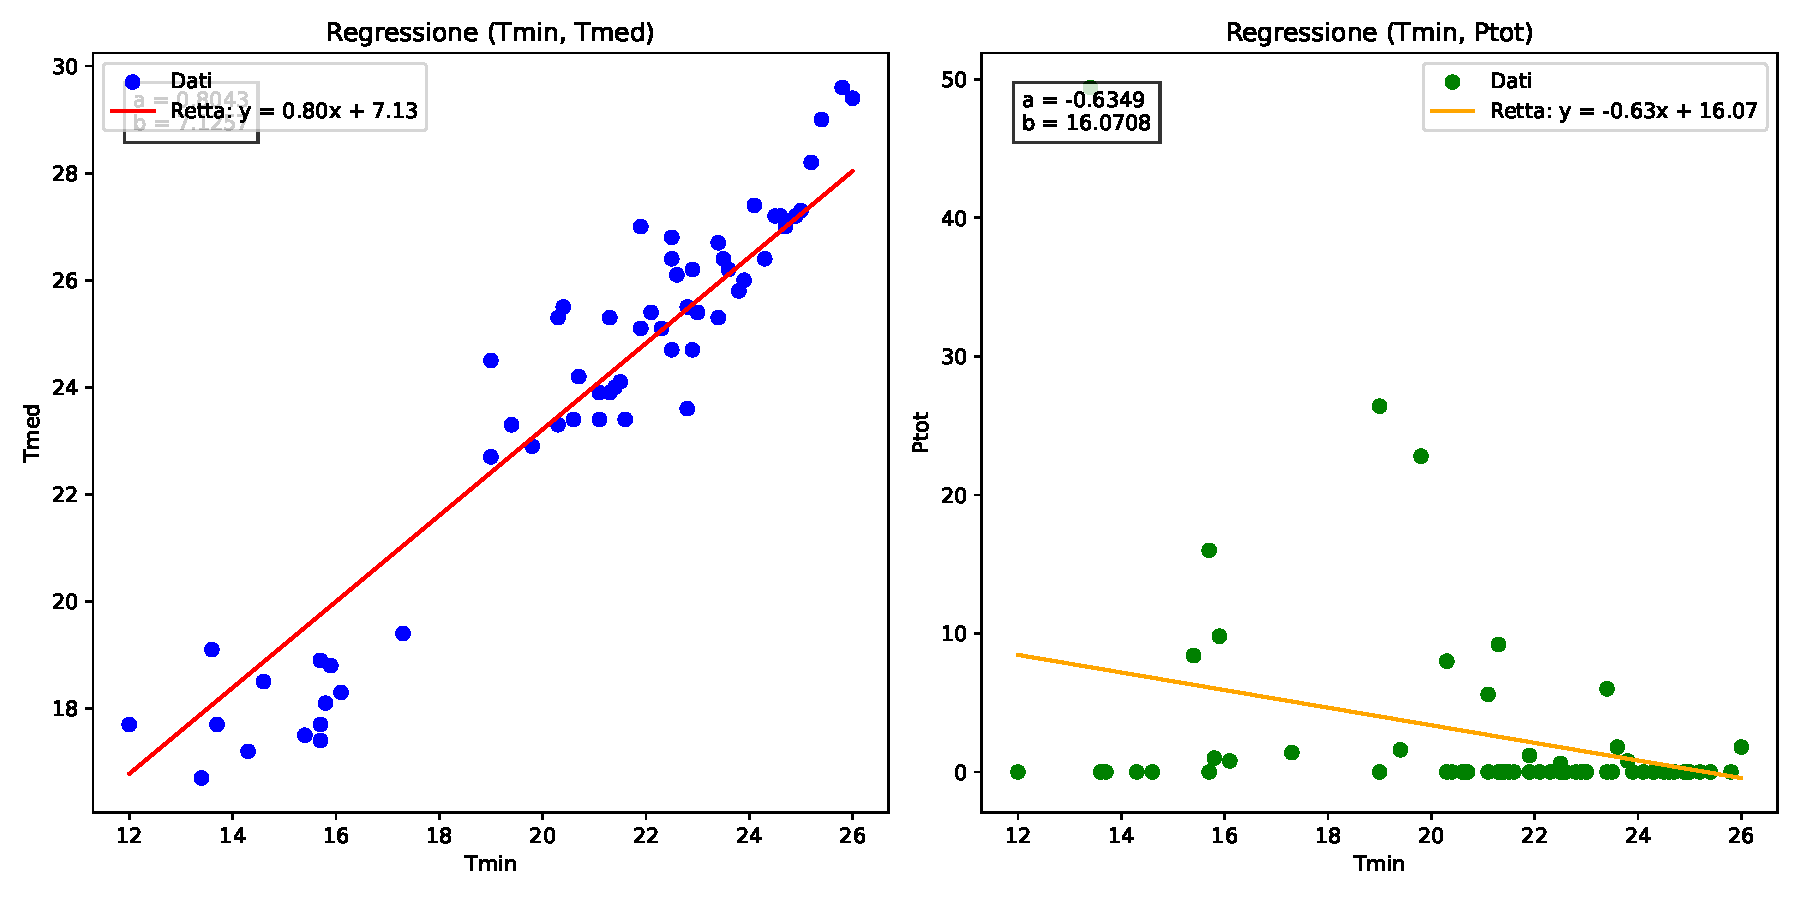
\includegraphics[width=0.8\textwidth]{gradient_descent_regression_plots.pdf}
    \caption{Diagrammi di dispersione con le rette di regressione ottenute tramite Gradient Descent.}
\end{figure}

I valori ottimali dei coefficienti sono:
\[
\text{Punto di minimo per } (Tmin, Tmed): a^* = \texttt{0,8043}, b^* = \texttt{7,125}
\]
\[
\text{Punto di minimo per } (Tmin, Ptot): a^* = \texttt{-0,6349}, b^* = \texttt{16,0708}
\]

\section{Conclusioni}
Il Gradient Descent è un metodo efficace per trovare il minimo della funzione di errore quadratico medio nella regressione lineare. La scelta del learning rate \(\alpha\) e del numero di iterazioni \(T\) è cruciale per garantire una convergenza rapida e stabile.



\end{document}